% !TEX encoding = UTF-8 Unicode
%%%%%%%%%%%%%%%%%%%%%%%%%%%%%%%%%%%%%%%%%
% Requisitos del protocolo de descubrimiento de servicios a crear
% 
% Autoría original:
% Linux and Unix Users Group at Virginia Tech Wiki 
% (https://vtluug.org/wiki/Example_LaTeX_chem_lab_report)
% Proporcionada por http://www.LaTeXTemplates.com
%
% Licencia:
% CC BY-NC-SA 3.0 (http://creativecommons.org/licenses/by-nc-sa/3.0/)
%
%%%%%%%%%%%%%%%%%%%%%%%%%%%%%%%%%%%%%%%%%

%----------------------------------------------------------------------------------------
%	PACKAGES AND DOCUMENT CONFIGURATIONS
%----------------------------------------------------------------------------------------

\documentclass{article}
\newcommand{\titulo}{x : Protocolo de descubrimiento de servicios}
\newcommand{\autor}{Diego Martín Arroyo}
\newcommand{\nombre}{Patata}



\usepackage{graphicx} % Requerido para la inclusión de imágenes
\usepackage{listings} % Requerido para la inserción de código
\usepackage[numbers]{natbib} % Requerido para cambiar el estilo de la bibliografía a APA. [numbers] para eliminar problemas de compatibilidad. Ver http://www.multiasking.com/blog/package-natbib-error-bibliography-not-compatible-with-author-year-citation/


\usepackage[T1]{fontenc} % Codificación de las fuentes utilizadas
%\usepackage[utf8]{inputenc} % Codificación de caracterers de entrada en UTF-8 (necesario para los caraceteres propios del español). Comentado dado que es ignorado con el compilador de XeLaTeX
\usepackage[spanish]{babel} % Español como idioma principal del texto (permite hyphenation de palabras al final de una línea)

\usepackage{courier} % Requerido para el uso de la fuente Courier
\usepackage[usenames,dvipsnames]{color} % Requerido para el uso de colores

%Metadatos del PDF e inclusión de referencias "clicables"
\usepackage[pdfauthor={\autor},
            pdftitle={\titulo},
            pdfproducer={XeLaTeX with hyperref},
            pdfcreator={XeLaTeX}]{hyperref}

\usepackage{url}
\usepackage{float} % Requerido para el posicionamiento absoluto de las imágenes. Ver http://en.wikibooks.org/wiki/LaTeX/Floats,_Figures_and_Captions
\usepackage[raggedright]{titlesec} % Evita la unión con guión de los \(sub)*section. Ver http://tex.stackexchange.com/questions/24777/how-to-disable-hyphenation-in-all-section-and-subsection-titles
%And if You used titleformat from titlesec to style titles -- You can do it explicitly: \titleformat{\section}{\color{teal}\LARGE\raggedright}{\hspace{0.5cm}\thetitle\‌​hspace{0.5cm}}{0cm}{} (note the \raggedright)

%\usepackage{titlesec}
%\newcommand{\sectionbreak}{\clearpage} % See http://tex.stackexchange.com/questions/9497/start-new-page-with-each-section

% Márgenes
\topmargin=-0.45in
\evensidemargin=0in
\oddsidemargin=0in
\textwidth=6.5in
\textheight=8.5in
\headsep=0.25in

\graphicspath{{./img/}}
\selectlanguage{spanish}

\newcommand*\lstinputpath[1]{\lstset{inputpath=#1}}

%\setlength\parindent{0pt} % Removes all indentation from paragraphs

%\renewcommand{\labelenumi}{\alph{enumi}.} % Descomentar para que la enumeración en el entorno enumerate sea mediante letras en vez de números




%Lenguajes de los que mostrar código
\lstloadlanguages{Java,XML,Python,JavaScript}

%Ajustes para Java
\lstset{
    language=java,
    frame=single, % Un marco simple alrededor del código
    basicstyle=\small\ttfamily, % Utilizar fuente true type pequeña
    keywordstyle=[1]\color{Blue}\bf, % Funciones en negrita y azul
    keywordstyle=[2]\color{Purple}, % Argumentos en morado
    keywordstyle=[3]\color{Blue}\underbar, % Funciones personalizadas subrayadas en azul
    identifierstyle=, % Nada especial acerca de identificadores
    commentstyle=\usefont{T1}{pcr}{m}{sl}\color{Green}\small, % Los comentarios se renderizan en fuente pequeña verde
    stringstyle=\color{Purple}, % Cadenas en morado
    showstringspaces=false, % No se muestran los espacios entre cadenas
    tabsize=5, % 5 espacios por tabulado
    %
    % Put standard Perl functions not included in the default language here
    %morekeywords={rand},
    %
    % Put Perl function parameters here
    %morekeywords=[2]{on, off, interp},
    %
    % Put user defined functions here
    %morekeywords=[3]{test},
   	%
    morecomment=[l][\color{Blue}]{...}, % Line continuation (...) like blue comment
    numbers=left, % Número de línea a la izquierda
    firstnumber=1, % Número de línea comienza en 1
    numberstyle=\tiny\color{Blue}, % Los números de línea son azules y pequeños
    stepnumber=5, % Los números de línea van de 5 en 5
    breaklines=true % Salto de línea si el texto no entra. See http://stackoverflow.com/a/1875803
}

%\usepackage{times} % Uncomment to use the Times New Roman font

%----------------------------------------------------------------------------------------
%	DOCUMENT INFORMATION
%----------------------------------------------------------------------------------------

\title{\titulo}
\author{\autor}
\date{\today} % Fecha

\lstinputpath{../../src/}

\newcommand{\javacode}[4]{
	\lstinputlisting[caption=#2,label=#1, firstline=#3, lastline=#4]{#1.java}
}

\newcommand{\txtcode}[4]{
	\lstinputlisting[caption=#2, label=#1, firstline=#3, lastline=#4]{#1.txt}
}

\newcommand{\pythoncode}[4]{
	\lstinputlisting[caption=#2, label=#1, firstline=#3, lastline=#4]{#1.py}
}

\begin{document}

\maketitle

\begin{abstract}
El protocolo \nombre permite el descubrimiento de máquinas ofreciendo una serie de servicios consumibles por el sistema distribuido, permitiendo publicar y solicitar nodos, obtener información del estado de nodos y una serie de funcionalidades de diagnóstico.
\end{abstract}

\section{Motivación}

El protocolo surge de la necesidad de minimizar la configuración manual que debe realizar un administrador en cada nodo y las ventajas que ofrece la inserción automática de 

%
%%----------------------------------------------------------------------------------------
%%	SECTION 1
%%----------------------------------------------------------------------------------------
%
\section{Enunciado}

Esta práctica implementa el algoritmo de filtrado de pares de NTP en un despliegue de varias máquinas, utilizando servicios web para la comunicación entre procesos y máquinas. La práctica consiste en la implementación del Algoritmo de Marzullo \cite{marzullo84}. Se simularán retardos en el cálculo del tiempo para la simulación de un equipo con cierto retardo entre la llegada de una petición y el envío de una respuesta.

%%%----------------------------------------------------------------------------------------
%%%	SECTION 2
%%%----------------------------------------------------------------------------------------

%\newpage
\section{Planteamiento de la solución}

Se propone la siguiente solución al problema planteado por el profesor:

\begin{itemize}
  \item Una clase \verb+Servidor+ que atienda peticiones HTTP sobre el reloj del servidor. Existirá una instancia de este proceso por cada máquina.
  \item Una clase \verb+NTP+ que consulta los tiempos a todas las máquinas y calcula el \textit{offset} (desvío) y el \textit{delay} (retardo) de la máquina respecto al reloj interno.
\end{itemize}

\subsection{Clase Servidor}

La clase \verb+Servidor+ proporciona servicios web en las rutas \verb+rest/tiempo+ y \verb+datos+ sobre su tiempo interno. Se simula un retardo entre los tiempos de llegada de una petición y el envío de la información utilizando la el método \textit{sleep} de la clase \verb+Thread+.

\javacode{net/martinarroyo/ntp/Servidor}{El servicio atiende las peticiones y genera una respuesta con un retardo entre 1 y 4 segundos.}{31}{50}

Una vez que la clase \verb+NTP+ que se encarga de calcular las diferencias de tiempo entre el servidor y esta, envía la información sobre el \textit{offset} y el \textit{delay} mediante una petición POST codificados en un formulario.

\javacode{net/martinarroyo/ntp/Servidor}{El método procesa los datos recibidos y los almacena para poder utilizarlos posteriormente}{99}{103}

Debido al uso de la etiqueta \verb+@Singleton+ los datos se almacenan y se puede acceder a ellos posteriormente en una interfaz web.

\begin{figure}[H]
   \begin{center}
   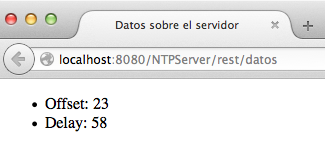
\includegraphics[width=0.4\textwidth]{interfazWeb}
   \caption{Visualización de los datos sobre el \textit{offset} y el \texit{delay}}
   \end{center}
\end{figure} 

\subsection{Clase NTP}

La clase NTP se encarga de preguntar a los servidores por el tiempo de cada \verb+Servidor+ y de calcular el retardo de estos mediante el algoritmo de Marzullo. Utiliza peticiones HTTP a los servicios descritos anteriormente y una serie de estructuras para almacenar la información.

Debido a que se deben realizar 8 peticiones por \verb+Servidor+, y que el tiempo mínimo de proceso de cada una es de un segundo, se ha apostado por la paralelización mediante hilos del cálculo de cada máquina.


\javacode{net/martinarroyo/ntp/Ntp}{Método main de la clase, encargado de leer de un fichero las direcciones a las que conectarse y realizando la invocación de los hilos}{35}{62}

\javacode{net/martinarroyo/ntp/Ntp}{Ejecución de cada hilo en el método run}{78}{103}

\subsection{Clase Tiempo}

El intercambio de información se realiza mediante instancias de la clase \verb+Tiempos+, que ha sido configurada para poder ser enviada como XML entre procesos utilizando la etiqueta \verb+@XmlRootElement+.

\javacode{net/martinarroyo/ntp/Tiempos}{Vista de los campos de información de la clase Tiempos}{5}{10}

\section{Despliegue y evaluación de la viabilidad del sistema para su utilización en esta práctica}

El despliegue se ha realizado directamente en el sistema Raspberry Pi, sobre Tomcat 7 y ArchLinux ARM con la JVM OpenJDK 8.

Debido a que aún no se cuenta con todos los componentes del sistema, los resultados de estas pruebas no determinan de forma precisa la viabilidad que se pretende evaluar. Sin embargo, como se indica posteriormente, es posible utilizar los resultados de esta evaluación como estimación válida de dicha viabilidad.

El sistema utilizado para realizar las pruebas consiste en:

\begin{itemize}
   \item Una Raspberry Pi 1 B de Primera Generación con el sistema operativo ArchLinux ARM y la máquina virtual de Java OpenJDK versión 1.8, ejecutando Tomcat 7 como servidor web. 
   \item Una Raspberry Pi 2 B de Primera Generación con el sistema operativo ArchLinux ARM y la máquina virtual de Java OpenJDK versión 1.8, corriendo Tomcat 7 como servidor web.
   \item Equipo de escritorio ejecutando la JVM 1.8 de Oracle.
   \item Cableado Ethernet que conecta todos los equipos a la misma subred (con un \textit{switch} que las conecta directamente).
\end{itemize}


\begin{figure}[H]
  \begin{center}
    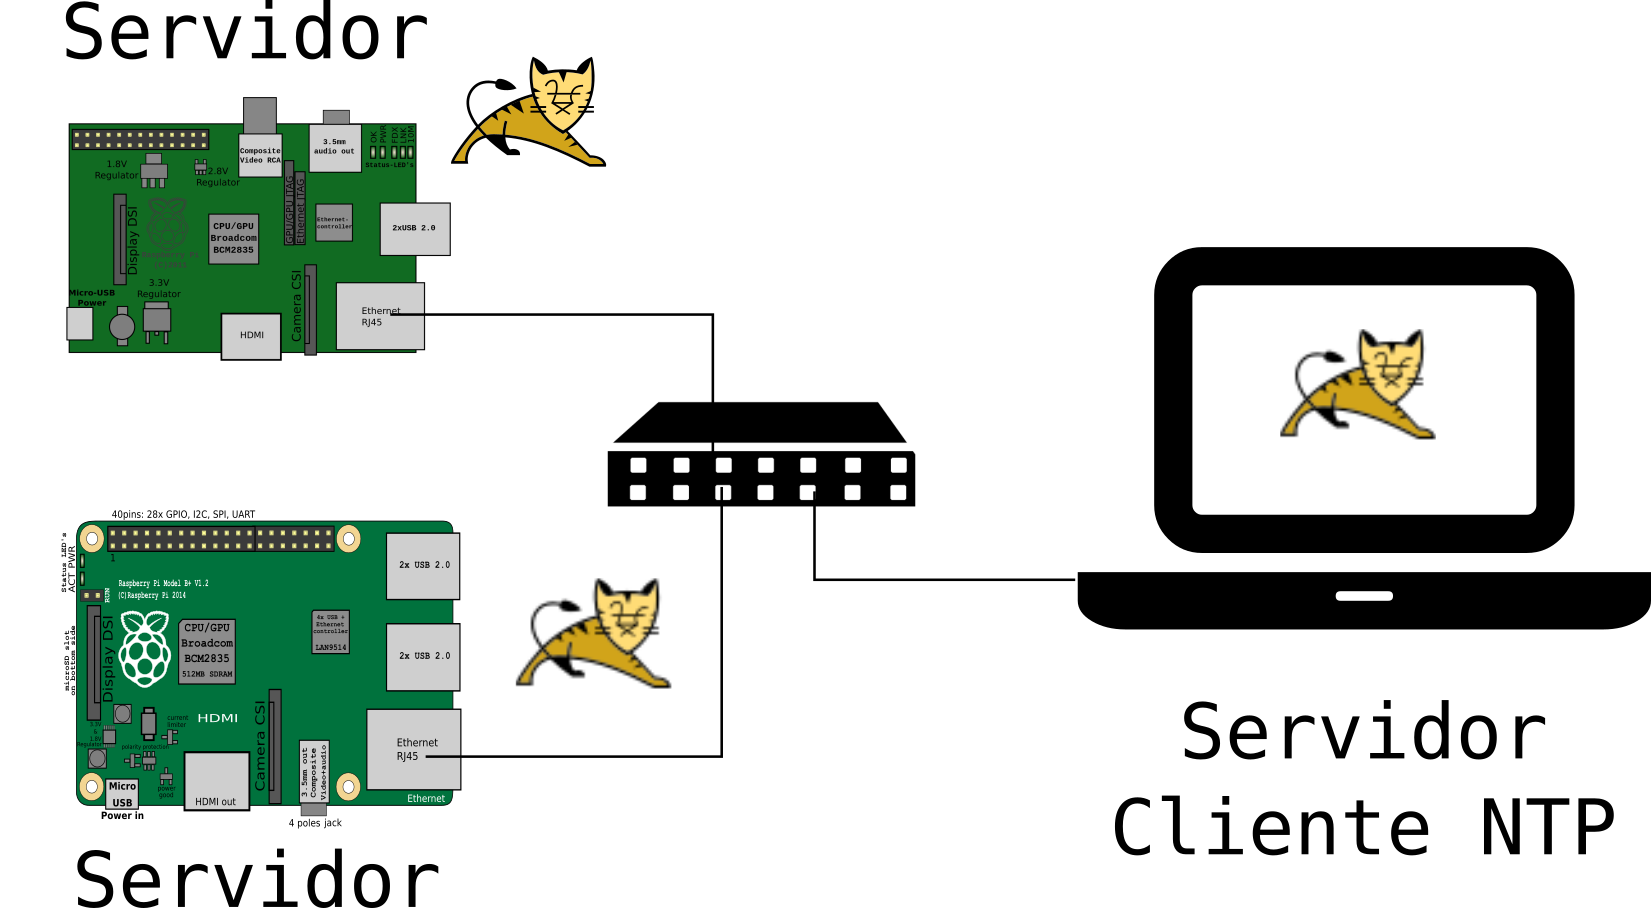
\includegraphics[width=0.4\textwidth]{arquitectura}
    \caption{Esquema sencillo de la arquitectura del despliegue}
  \end{center}
\end{figure}

\subsection{Evaluación del rendimiento}

Todo el código de Tomcat se ejecuta sobre la máquina virtual de Java, cuyo consumo de recursos puede ser significativo en ocasiones. Este problema es particularmente acuciante en sistemas embebidos como el sujeto de pruebas en cuestión. Con el objetivo de mejorar el rendimiento se ha utilizado la biblioteca opcional de Tomcat \verb+tomcat-native+, que permite a Tomcat utilizar ciertos recursos nativos a través de la \textit{Apache Portable Runtime} (APR) \cite{tomcatnative}.

Observando el comportamiento de Tomcat al arrancar y solicitar una serie de servicios, se observa un gran retardo a la hora de realizar la primera solicitud (que implica la carga de los recursos que cada programa demande) y en el arranque del servidor. Sin embargo, las posteriores invocaciones a los servicios web evaluados (implementación del ejercicio planteado) reflejan tiempos de respuesta similares a los de un equipo de escritorio (tiempos de respuesta casi instantáneos). Dicho comportamiento es similar al descrito en prácticas anteriores.

No obstante, se observa una mejora de rendimiento al utilizar el modelo 2 de Raspberry Pi.

\begin{figure}[H]
 \txtcode{../doc/tex/slow}{File}{1}{8}
 \caption{Primera consulta utilizando la herramienta cURL \cite{cURLPerformance}}
\end{figure}
\begin{figure}[H]
 \txtcode{../doc/tex/fast}{File}{1}{8}
 \caption{Segunda consulta utilizando la herramienta cURL \cite{cURLPerformance}} 
\end{figure}

\subsection{Evaluación de la experiencia de uso}

Se ha solicitado a varios estudiantes de la asignatura sistemas distribuidos que prueben su solución a la práctica en el sistema.

\subsection{}

%
%Utilizando la Raspberry Pi como servidor se ha conseguido la comunicación entre los dos nodos y la simulación de carreras con 4 atletas con un rendimiento similar al obtenido en las pruebas con un único nodo. Si bien el tiempo de carga inicial de los datos en la \textit{JVM} dificulta la realización de pruebas que impliquen el reinicio o recarga del servidor, el sistema es capaz de reemplazar a los equipos del laboratorio para la ejecución de las versiones definitivas del código.
%
%\subsection{\textit{Deployment} del código}
%
%Debido a la portabilidad del código Java, es posible realizar una compilación y empaquetado del código en una unidad (archivo) portable entre máquinas con diferentes arquitecturas.
%
%(Por completar)
%%Para ello se ha modificado el \textit{script} proporcionado por el profesor para automatizar la tarea de instalación del código en diferentes máquinas pertenecientes a la misma red. Para hacer aún más sencillo el proceso, se utiliza autenticación por clave pública en detrimento de la autenticación mediante contraseña.
%
%%El código del servicio web se instala mediante la creación de un archivo \verb+.war+ y posterior \textit{deployment} utilizando el script pertinente o la interfaz web proporcionada por Tomcat.
%
%\subsection{Evaluación de alumnos}
%(Por realizar)
%%TODO: Realizar
%
%\subsection{Conclusiones}
%
%En virtud de lo expuesto en esta sección, la viabilidad de la realización de esta práctica en el futuro sistema es factible, máxime cuando aún no se cuenta con los componentes definitivos, cuyo rendimiento es mucho mayor que el sistema en el que se han realizado las pruebas. Existen además opciones para realizar una ejecución del código de forma mucho más óptima, como el paquete \verb+tomcat-native+ \cite{TomcatNative}


%%	BIBLIOGRAPHY
%%----------------------------------------------------------------------------------------
%

\bibliographystyle{ieeetr}
%
\bibliography{ntpserver}
%%----------------------------------------------------------------------------------------
%

\end{document}
